\documentclass[preprint,12pt]{elsarticle}

\usepackage{amsmath,amssymb}
\usepackage{booktabs}
\usepackage{array}
\usepackage{graphicx}
\usepackage{multirow}
\usepackage{siunitx}
\usepackage{url}
\usepackage{xcolor}
\usepackage{microtype}
\usepackage{enumitem}
\usepackage{threeparttable}
\usepackage{algorithm}
\usepackage{algpseudocode}
\usepackage[hidelinks]{hyperref}

\journal{Results in Engineering}
\emergencystretch=2em
\renewcommand{\topfraction}{0.9}
\renewcommand{\bottomfraction}{0.8}
\renewcommand{\textfraction}{0.07}
\renewcommand{\floatpagefraction}{0.75}
\setcounter{topnumber}{3}
\setcounter{bottomnumber}{2}
\setcounter{totalnumber}{5}
\biboptions{sort&compress}

\begin{document}

\begin{frontmatter}

\title{AudioTwin: Preference-Guided Personalisation of Hearing-Aid Signal Processing with Constrained Bayesian Optimisation}

\author[anon]{Anonymous Author}
\address[anon]{Anonymous Institution}

\begin{abstract}
A practical problem in hearing-aid fitting is that a clinically reasonable starting setting may still not match what an individual listener finds clear, comfortable and acceptable in daily use. Fine-tuning can therefore require repeated manual adjustments, while each extra listening judgement adds time and effort for the user. This study presents \textit{AudioTwin}, a simulation framework that treats hearing-aid personalisation as a constrained engineering optimisation problem. The system starts from audiogram information, asks the listener to choose between pairs of feasible settings, learns from these choices using a Gaussian-process preference model, and uses expected utility of the best option (qEUBO) to select the next comparison. The processing space covers gain, spectral tilt, compression, noise reduction, speech enhancement and compression speed. In a frozen evaluation of 128 simulated listeners across three listening contexts and three pre-specified preference families, qEUBO reduced mean normalised regret from 0.321 for the best static fitting to 0.240 after 20 comparisons, a 25.1\% reduction; 94 of 128 listeners improved. Targeted query selection also outperformed matched random querying after only five comparisons. The engineering contribution is a reproducible way to combine measured hearing information, individual preference and constrained device control in one loop. If confirmed with human listeners, this approach could reduce unnecessary fine-tuning steps, support more individualised fittings and help hearing devices adapt more efficiently to different listening needs. The present evidence is computational and does not establish clinical benefit or medical-device safety.
\end{abstract}

\begin{keyword}
biomedical signal processing \sep hearing aid \sep closed-loop control \sep preferential Bayesian optimisation \sep audiometry \sep personalised assistive devices \sep active learning
\end{keyword}

\end{frontmatter}

\section{Introduction}
\label{sec:introduction}

Hearing aids are normally fitted from measured hearing loss and established prescription rules. This provides an important starting point, but it does not fully capture what an individual listener finds clear, comfortable or natural. Two people with similar audiograms can prefer different gain, compression or noise-processing settings. In practice, this can lead to repeated fine-tuning, extra clinic time and settings that work well in one situation but less well in another. The real-world engineering problem is therefore not only to produce a technically valid fitting, but to reach a useful individual setting with as little user effort as possible.

A practical personalisation system should learn from the listener without requiring long questionnaires or many manual adjustments. Pairwise choices offer a simple form of feedback: the user listens to two feasible settings and selects the one they prefer. The challenge is to decide which comparison should be asked next. Random or poorly chosen comparisons can waste limited attention, while repeated judgements can become less reliable as the listener becomes tired. An efficient system should therefore use each response to improve the final recommendation as much as possible.

Bayesian optimisation (BO) is designed for problems where evaluating a candidate is costly \cite{shahriari2016}. Preferential Bayesian optimisation (PBO) extends this idea to comparative feedback such as ``setting $i$ is preferred to setting $j$'' \cite{gonzalez2017}. Gaussian-process (GP) preference learning provides a probabilistic model of the listener's latent preference from these comparisons \cite{chu2005,rasmussen2006}. The acquisition rule then decides which pair of settings should be compared next.

Hearing-aid fitting is a suitable application for this approach. Prescriptive methods such as NAL-NL2 provide a principled starting response from audiometric information \cite{keidser2011}, but they cannot represent every personal preference. Previous studies show that listeners can make systematic self-adjustments \cite{dreschler2008,boothroyd2017,mackersie2019,sabin2020}, and preference-based learning has been explored for hearing-aid personalisation \cite{birlutiu2010,nielsen2015,vyas2022,akbarzadeh2022,ni2024}. However, a useful engineering system must do more than learn preference. It must keep proposed settings within defined operating limits, use a small number of interactions and be tested against strong static alternatives.

This paper presents \textit{AudioTwin}, a reproducible closed-loop framework for preference-guided hearing-aid personalisation. The system combines an audiogram-conditioned device model, a simulated listener and a preference-learning controller. A six-dimensional control vector changes gain, spectral tilt, compression, noise reduction, speech enhancement and compression speed. The controller learns from binary choices using a Laplace-approximated GP preference model. Expected utility of the best option (qEUBO) selects the next pair to compare \cite{astudillo2023}, and every candidate is projected into a deterministic feasible region before it can be queried or recommended.

The main practical change introduced by AudioTwin is that fine-tuning is treated as an active learning process rather than a sequence of manual trial-and-error adjustments. The system tries to ask only comparisons that are useful for the final decision. If this behaviour transfers to real listeners, it could reduce the number of adjustments needed to reach a preferred setting, reduce unnecessary user effort and support more responsive fitting across listening situations. It could be used as a clinician-assisted tool or, after appropriate validation and regulatory work, as part of a guided self-fitting workflow. This study does not claim these clinical benefits have already been achieved; it tests the engineering principle in a controlled simulation before human evaluation.

The term \emph{safety-constrained} is used here only in a computational sense. Known model-based bounds, output limits and adjacent-band gain-smoothness constraints are enforced by construction. This is different from methods such as SafeOpt that learn an unknown safety function under uncertainty \cite{sui2015}. The constraints in AudioTwin are engineering guardrails in the simulator and are not medical-device safety certification.

\begin{figure}[!htbp]
\centering
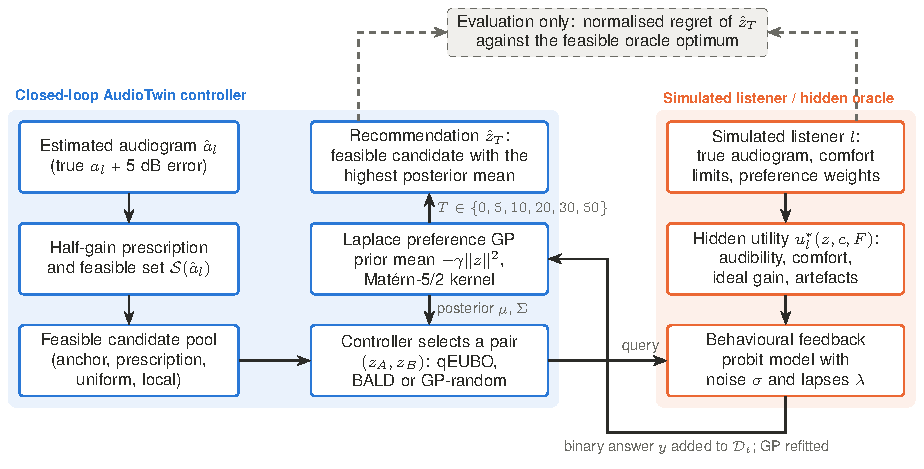
\includegraphics[width=\linewidth]{fig1_framework.pdf}
\caption{Closed-loop AudioTwin architecture. An estimated audiogram defines the feasible hearing-aid processing space. The controller presents a pair of feasible settings, receives a binary preference from the simulated listener, updates the preference model and recommends the setting with the highest posterior mean utility. The hidden oracle is used only to generate simulated feedback and evaluate recommendations.}
\label{fig:framework}
\end{figure}

The study addresses four questions:
\begin{enumerate}[label=(Q\arabic*)]
    \item Can a small number of preference comparisons improve an audiogram-initialised static fitting?
    \item Does targeted query selection improve the final recommendation compared with random comparisons using the same preference model?
    \item How does performance change across listening contexts and preference families?
    \item Can deterministic feasibility constraints and a frozen evaluation protocol provide a reproducible benchmark for adaptive hearing-aid control?
\end{enumerate}

The main contributions are:
\begin{itemize}
    \item a closed-loop engineering formulation that joins audiogram information, listener preference feedback and adaptive control of six hearing-aid processing dimensions;
    \item an audiogram-conditioned feasible processing space covering gain, spectral tilt, compression, noise reduction, speech enhancement and compression speed;
    \item a matched comparison of qEUBO, BALD and random pair acquisition using the same GP model, candidate generator and common random-number seeds;
    \item a conservative static reference and a frozen final evaluation with a reserved seed, pre-specified primary endpoint, listener-level bootstrap inference and an explicit infeasibility rule;
    \item an open and reproducible simulation package that can be used to study query efficiency, response reliability and failure modes before a human-listener study.
\end{itemize}

The final evaluation contains 128 independent simulated listeners. The pre-specified primary hypothesis is that AudioTwin-qEUBO at 20 comparisons has lower normalised regret than the best static comparator. Secondary analyses examine query efficiency against random pair selection, BALD, larger budgets, context and preference-family differences, and a separately labelled post-hoc robustness family. Section~\ref{sec:exploratory} reports exploratory analyses completed after the frozen evaluation.

\section{Related work}
\label{sec:related}

\subsection{Preferential Bayesian optimisation}

A pairwise preference $x_i \succ x_j$ can be represented through a latent utility function $f$ with $f(x_i)>f(x_j)$. Chu and Ghahramani \cite{chu2005} introduced a GP framework for learning such latent preference functions from comparison data. A GP prior supplies a smooth probabilistic function model, and a non-Gaussian pairwise likelihood maps utility differences to comparison probabilities. Approximate posterior inference is then required, commonly via Laplace or expectation-propagation methods.

PBO extends this model from prediction to sequential decision making \cite{gonzalez2017}. At each iteration, the learner chooses a pair of alternatives, observes the user's preference, updates the posterior and ultimately recommends a configuration. Selection policies can target uncertainty, information gain or decision quality. BALD is an information-theoretic active-learning strategy based on expected information gain \cite{houlsby2011}. Ignatenko et al. \cite{ignatenko2025} formulate user preference learning as sequential BO with pairwise comparisons, choosing proposals that reduce uncertainty about the user's responses. Preference exploration has also been combined with BO over multiple outcomes \cite{lin2022}. qEUBO instead scores a candidate set by its expected utility of the best option and is derived directly from the terminal decision objective \cite{astudillo2023}; Astudillo et al. showed that it has a simple computational form and favourable simple-regret behaviour under appropriate assumptions.

Safety-aware BO is a related but distinct literature. SafeOpt, for example, expands a set of points whose unknown safety value is inferred with a GP while maintaining probabilistic safety guarantees \cite{sui2015}. In AudioTwin, the relevant constraints are deterministic functions of the estimated listener state and DSP configuration. The learner therefore searches only over projected feasible settings rather than learning whether a queried point is safe.

\subsection{Adaptive hearing-aid signal processing and personalisation}

Population-derived prescriptions are an important starting point in hearing-aid fitting, but they cannot encode every listener's subjective preference. NAL-NL2 combines audiometric information with models of speech intelligibility and loudness to derive frequency-dependent targets \cite{keidser2011}. User-directed adjustment studies nevertheless demonstrate residual individual preference variation. Dreschler et al. \cite{dreschler2008} reported systematic client-controlled gain adjustments, while the ``Goldilocks'' studies showed that users can navigate low-dimensional self-fitting controls and obtain plausible gain responses \cite{boothroyd2017,mackersie2019}. Sabin et al. \cite{sabin2020} evaluated a self-fitting interface that jointly adjusted gain and compression in real-world use.

Machine-learning approaches aim to make this preference elicitation more efficient (Table~\ref{tab:prior}). Birlutiu et al. \cite{birlutiu2010} used multi-task GP preference learning on pairwise sound-quality data, showing that structure shared across users can improve prediction. Nielsen et al. \cite{nielsen2015} are particularly close to the present work: they combined Gaussian processes, active learning and pairwise perceptual comparisons to personalise up to four hearing-aid parameters with hearing-aid users. Korzepa et al. \cite{korzepa2020} proposed a simulation environment for contextual hearing-aid personalisation in which synthetic users rate settings on a slider. Alamdari et al. \cite{alamdari2020} personalised compression by human-in-the-loop deep reinforcement learning, and Akbarzadeh et al. \cite{akbarzadeh2022} learned compression preferences by maximum-likelihood inverse reinforcement learning from pairwise comparisons against prescriptive settings. Vyas et al. \cite{vyas2022} reduced a 24-dimensional configuration space to a set of presets and used online learning over pairwise comparisons. Ni et al. \cite{ni2024} proposed efficient multi-band Bayesian learning, with simulation evidence and a small clinical experiment.

\begin{table}[!htbp]
\centering
\caption{Representative machine-learning approaches to hearing-aid personalisation from user feedback.}
\label{tab:prior}
\small
\begin{tabular}{@{}>{\raggedright\arraybackslash}p{0.205\linewidth}>{\raggedright\arraybackslash}p{0.18\linewidth}>{\raggedright\arraybackslash}p{0.31\linewidth}>{\raggedright\arraybackslash}p{0.21\linewidth}@{}}
\toprule
Study & Feedback & Learning approach & Evaluation \\
\midrule
Birlutiu et al.~\cite{birlutiu2010} & Pairwise & Multi-task GP preference learning & Offline prediction on listener data \\
Nielsen et al.~\cite{nielsen2015} & Pairwise perceptual & GP with active learning; up to four parameters & Hearing-aid users \\
Korzepa et al.~\cite{korzepa2020} & Slider ratings & Contextual BO in a simulation environment & Simulated users \\
Alamdari et al.~\cite{alamdari2020} & User feedback & Human-in-the-loop deep RL for compression & Subject testing \\
Akbarzadeh et al.~\cite{akbarzadeh2022} & Pairwise vs.\ prescription & Maximum-likelihood inverse RL for compression & Ten subjects \\
Vyas et al.~\cite{vyas2022} & Pairwise & Online learning over presets & Simulation and participant data \\
Ni et al.~\cite{ni2024} & User feedback & Multi-band Bayesian learning & Simulation; eight subjects \\
AudioTwin (this work) & Noisy pairwise (simulated) & Constrained PBO; matched qEUBO, BALD and random acquisition & 128 simulated listeners; frozen protocol \\
\bottomrule
\end{tabular}
\end{table}

AudioTwin is complementary to these studies rather than a replacement for them. Its methodological focus is the joint evaluation of (i) continuous latent control across multiple DSP dimensions, (ii) deterministic feasibility constraints, (iii) decision-theoretic active acquisition, (iv) matched acquisition ablations, and (v) a leakage-resistant final protocol. In particular, the qEUBO comparison asks whether an explicit decision-theoretic acquisition policy improves recommendations relative to random querying when all other modelling choices are held fixed.

\section{Closed-loop problem formulation}
\label{sec:problem}

The adaptive loop receives two forms of listener information: an estimated audiogram $\hat a_l$, which conditions admissible device settings, and sequential binary perceptual responses, which update the preference model. Let $z\in\mathcal Z\subset[-1,1]^6$ denote a latent hearing-aid DSP control vector and $c\in\mathcal C$ a listening context. For listener $l$, an unknown utility function
\begin{equation}
    u_l(z,c):\mathcal Z\times\mathcal C\rightarrow\mathbb R
\end{equation}
encodes preference. Direct utility observations are unavailable. Instead, a query presents two feasible settings $(z_A,z_B)$ and returns a binary preference $y\in\{A,B\}$.

The optimisation objective after $T$ comparisons is to recommend
\begin{equation}
    \hat z_T(c)=\arg\max_{z\in\mathcal S(\hat a_l)} \mathbb E[f_l(z,c)\mid\mathcal D_T],
    \label{eq:recommend}
\end{equation}
where $\hat a_l$ is an estimated audiogram, $\mathcal S$ is the deterministic feasible set, $f_l$ is the learned latent preference model, and $\mathcal D_T$ is the set of observed pairwise choices.

For evaluation only, a hidden oracle utility $u_l^*$ is available. Let $u^*_{l,c,F}$ be the feasible optimum for listener $l$, context $c$ and preference family $F$, and let $u^{\mathrm{lo}}_{l,c,F}$ be the 5th percentile of oracle utility over 400 uniformly sampled feasible settings. Normalised regret is
\begin{equation}
    r_T = \frac{\max\{u^*_{l,c,F}-u_l^*(\hat z_T,c,F),\,0\}}{u^*_{l,c,F}-u^{\mathrm{lo}}_{l,c,F}},
    \label{eq:regret}
\end{equation}
with lower values preferred. A value of one corresponds to a setting as poor as that low reference; values above one are possible (15 of the 32,256 final rows; maximum 1.17).

The primary study endpoint averages the nine pre-specified context/family cells within each listener before population-level inference. This keeps the listener as the statistical unit and prevents the many within-listener rows from being treated as independent observations.

\section{AudioTwin closed-loop framework}
\label{sec:framework}

\subsection{Biomedical input: listener audiogram and uncertainty}

Each simulated listener has a seven-frequency true audiogram
\begin{equation}
 a_l=[a_{250},a_{500},a_{1000},a_{2000},a_{4000},a_{6000},a_{8000}],
\end{equation}
plus upper comfort limits and latent preference parameters. The fitting system observes a perturbed estimate
\begin{equation}
    \hat a_l=\mathrm{clip}\!\left(5\,\mathrm{round}\!\left(\frac{a_l+\epsilon}{5}\right),\,0,\,100\right),\qquad \epsilon\sim\mathcal N(0,\sigma_a^2I),
    \label{eq:audiogram-noise}
\end{equation}
that is, the noisy threshold rounded to the 5-dB audiometric grid and clipped to 0--100 dB HL, with $\sigma_a=5$ dB in the final evaluation. The separation between $a_l$ and $\hat a_l$ prevents the optimiser from receiving the exact hidden listener state.

\subsection{Controlled variables: six-dimensional hearing-aid DSP space}

AudioTwin maps $z=(z_1,\ldots,z_6)$ to DSP controls. The dimensions represent overall gain offset, spectral tilt, compression-ratio scale, noise reduction, speech enhancement and compression speed. Gain is represented over ten bands centred at 250, 500, 750, 1000, 1500, 2000, 3000, 4000, 6000 and 8000 Hz.

For band $k$,
\begin{equation}
 g_k(z)=\mathrm{clip}\left(g^{Rx}_k(\hat a_l)+b_1z_1+b_2z_2\log_2(f_k/1000),0,g^{\max}_k\right).
 \label{eq:gain}
\end{equation}
The reported simulator does \emph{not} implement NAL-NL2. Its synthetic prescription is an explicit half-gain rule,
\begin{equation}
 g^{Rx}_k(a)=0.5\,\tilde a_k,
 \label{eq:halfgain}
\end{equation}
where $\tilde a_k$ is the audiometric threshold interpolated to the ten DSP bands. NAL-NL2 is cited only as clinical background. The hidden ideal-gain term in the oracle is intentionally related to the same simulator construction: $g^{ideal}_{l,k}=g^{Rx}_k(a_l)+\delta_{l,k}$, where $a_l$ is the listener's true audiogram and $\delta_{l,k}$ is a listener-specific random offset. The ideal curve is therefore not an independent prescription, and this shared structure is a limitation of the benchmark.
Compression ratio is controlled as
\begin{equation}
 CR_k(z)=\mathrm{clip}\left(CR^{Rx}_k 2^{2z_3},1,CR_{\max}\right),
 \label{eq:compression}
\end{equation}
so the lower extreme reaches linear processing. Noise-reduction and speech-enhancement strengths are $(z_4+1)/2$ and $(z_5+1)/2$. Attack/release timing is interpolated logarithmically through $z_6$, from 5/50~ms at $z_6=0$ to 50/500~ms at $z_6=1$ (and 0.5/5~ms at $z_6=-1$).

The latent parameterisation is deliberately compact. It is not intended to reproduce every proprietary hearing-aid algorithm; rather, it provides a heterogeneous continuous space in which preference learning must coordinate spectral, dynamic and enhancement controls. Because compression speed has no term in the three primary utility families (Section~\ref{sec:oracle}), $z_6$ is a nuisance dimension in the primary analysis: the learner searches six dimensions, five of which affect utility, with an isotropic kernel.

\begin{table}[!htbp]
\centering
\caption{Core simulator parameters used in the reported study. These are synthetic modelling assumptions rather than clinical prescription constants. The complete inventory, distributions and oracle equations are given in Appendix~\ref{app:oracle} and \texttt{docs/simulator\_parameters.md}.}
\label{tab:simparams}
\small
\begin{tabular}{p{0.48\linewidth}p{0.42\linewidth}}
\toprule
Quantity & Value \\
\midrule
Audiogram observation error & $\sigma_a=5$ dB; rounded to 5 dB; clipped to 0--100 dB HL \\
Accepted PTA4 range & 20--55 dB HL \\
Prescription gain & $0.5\times$ interpolated threshold \\
Gain offset / spectral tilt & 10 dB per unit $z_1$ / 6 dB octave$^{-1}$ per unit $z_2$ \\
Compression range & prescribed CR $\times 2^{2z_3}$, clipped to [1,4] \\
Output check & predicted band output $\le$100 dB SPL for a 65-dB-SPL input \\
MPO limiter & 105 dB SPL \\
Adjacent-band gain limit & 12 dB \\
Fast / slow attack-release & 5/50 ms; 50/500 ms \\
Choice noise / lapse rate & $\sigma\sim U(0.05,0.15)$ / $\lambda\sim U(0,0.05)$ per listener \\
GP prior mean / kernel & $-0.1\|z\|^2$ / isotropic Mat\'ern-5/2 \\
Query candidates & anchor, prescription, 192 uniform + 64 local \\
Recommendation candidates & 256 uniform + 256 local + queried points \\
Query checkpoints & 0, 5, 10, 20, 30, 50 \\
Bootstrap & 20,000 listener resamples; seed 20261011 \\
\bottomrule
\end{tabular}
\end{table}

\subsection{Deterministic feasible set}

All methods operate under the same model-based constraints. In the reported final active-learning loop, a setting is admissible only if it lies inside the latent box, respects the gain bounds induced by the parameterisation, keeps the predicted band output for a 65-dB-SPL reference input below the fixed 100-dB-SPL ceiling and satisfies the adjacent-band gain-difference limit. The resulting set is denoted $\mathcal S(\hat a_l)$. The codebase also contains an optional previous-setting change-rate check for a legacy projection utility, but the final qEUBO/BALD/random loop checks feasibility without a previous setting and therefore does \emph{not} enforce a sequential change-rate constraint.

A conservative low-gain anchor is located first. Candidate settings are then projected from that anchor into the feasible region. Static baselines undergo the same projection as learned methods. Consequently, neither the baseline nor AudioTwin is evaluated at an unprojected setting that violates the frozen model constraints.

This design separates feasibility from acquisition: qEUBO, BALD and random selection may choose only among settings that have already passed deterministic projection.

\subsection{Hidden preference oracle}
\label{sec:oracle}

The simulation oracle combines four components:
\begin{equation}
 u_l^*(z,c,F)=w_A A(z,c)-w_C P_C(z,c)-w_D P_D(z)-w_Q P_Q(z,c),
 \label{eq:oracle}
\end{equation}
where $A$ is an audibility/intelligibility-like term, $P_C$ penalises loudness discomfort, $P_D$ penalises deviation from a listener-specific ideal gain curve and $P_Q$ penalises processing and compression artefacts (equations in Appendix~\ref{app:oracle}). Weights vary by listener and preference family. In speech contexts, noise reduction and speech enhancement raise the effective signal-to-noise ratio at an artefact cost; in music they provide no benefit and their artefact cost is doubled, so the music optimum lies at the noise-reduction/speech-enhancement-off corner by construction.

Three families were defined before the final evaluation: \emph{intelligibility}, \emph{comfort} and \emph{balanced}. A fourth \emph{noise-sensitive} family includes extra compression-in-noise penalties and is reported only as a post-hoc robustness analysis because it was introduced after development diagnostics.

Preference observations include stochastic response noise. For candidates $z_A$ and $z_B$,
\begin{equation}
 P(A\succ B)=\frac{\lambda}{2}+(1-\lambda)\Phi\left(\frac{u_l^*(z_A)-u_l^*(z_B)}{\sqrt{2}\sigma}\right),
 \label{eq:oracle-choice}
\end{equation}
where $\lambda$ represents lapse-like random responses and $\sigma$ controls comparison noise.

The oracle is intentionally analytic and computationally inexpensive. It is a controlled benchmark for optimisation, not a validated model of human auditory perception. The implications of this distinction are addressed in Section~\ref{sec:limitations}.

\section{Preference model and acquisition}
\label{sec:model}

\subsection{Laplace GP preference model}

AudioTwin places a GP prior on latent utility,
\begin{equation}
 f(z)\sim\mathcal{GP}(m(z),k(z,z')).
\end{equation}
The prior mean
\begin{equation}
 m(z)=-\gamma\|z\|^2, \qquad \gamma=0.1,
\end{equation}
creates a soft pull towards the prescription origin without hard-coding a development-derived preferred setting.

The covariance is Mat\'ern-$5/2$:
\begin{equation}
 k(z,z')=\sigma_f^2\left(1+\sqrt{5}r+\frac{5r^2}{3}\right)e^{-\sqrt{5}r},
 \qquad r=\frac{\|z-z'\|}{\ell}.
 \label{eq:matern}
\end{equation}

For an observed comparison in which item $i$ is preferred to item $j$,
\begin{equation}
 P(i\succ j\mid f)=\Phi\left(\frac{f_i-f_j}{\sqrt{2}\sigma_n}\right).
 \label{eq:probit}
\end{equation}
This likelihood has no lapse term, a deliberate mild misspecification relative to the oracle in Eq.~\eqref{eq:oracle-choice}. The non-Gaussian posterior is approximated by a Laplace expansion about the MAP latent vector, and predictive covariance includes uncertainty propagated from the queried latent values. Hyperparameters are re-selected every five queries by maximising the Laplace-approximated marginal likelihood over a frozen grid: lengthscale $\{0.6,1.0,1.6\}$, signal variance $\{0.1,0.3,1.0\}$ and assumed preference-noise scale $\{0.05,0.10,0.20\}$.

\subsection{qEUBO}

For two posterior utilities $f_i$ and $f_j$, qEUBO with $q=2$ scores a pair by
\begin{equation}
 \alpha_{\mathrm{EUBO}}(i,j)=\mathbb E[\max(f_i,f_j)].
 \label{eq:eubo}
\end{equation}
For a jointly Gaussian posterior this expectation is available in closed form. If $d=\mu_i-\mu_j$ and
\begin{equation}
 \theta^2=C_{ii}+C_{jj}-2C_{ij},
\end{equation}
then with $\alpha=d/\theta$,
\begin{equation}
 \mathbb E[\max(f_i,f_j)] = \mu_i\Phi(\alpha)+\mu_j\Phi(-\alpha)+\theta\phi(\alpha).
 \label{eq:eubo-closed}
\end{equation}
The selected pair maximises Eq.~\eqref{eq:eubo-closed} among sufficiently separated feasible candidates.

\subsection{BALD and GP-random controls}

BALD approximates the mutual information between the comparison response and the latent preference function \cite{houlsby2011}. It provides an uncertainty-centred active policy with the same posterior model as qEUBO.

GP-random is a stronger control than an unmodelled random baseline. It fits the identical Laplace GP and uses the same candidate pools, minimum separation logic and recommendation rule, but selects admissible query pairs uniformly at random. qEUBO--GP-random differences therefore isolate the effect of acquisition more cleanly than qEUBO--static comparisons alone.

\subsection{Candidate pools and recommendation}

At each interaction the candidate pool contains the conservative anchor, the safely projected prescription, uniform feasible samples and local samples around the current posterior incumbent. At evaluation checkpoints the recommendation is the feasible candidate with highest posterior mean. Budgets are $T\in\{0,5,10,20,30,50\}$. Algorithm~\ref{alg:loop} summarises one episode.

At $T=0$ the recommendation is exactly the safely projected prescription. This creates an intentionally conservative starting point: any subsequent benefit must be learned from preferences rather than inherited from a hand-crafted initial configuration.

\begin{algorithm}[!htbp]
\caption{One AudioTwin episode for listener $l$, context $c$ and family $F$}
\label{alg:loop}
\begin{algorithmic}[1]
\Require estimated audiogram $\hat a_l$, budget $T$, checkpoints $\mathcal K$, acquisition $\in\{$qEUBO, BALD, random$\}$
\State find a feasible low-gain anchor $z_0$; if none exists, stop (infeasible draw)
\State $z_{Rx}\gets$ projection of the prescription $z=0$ towards $z_0$; \ $\mathcal D\gets\emptyset$
\For{$t=0,1,\ldots,T$}
  \State fit the Laplace preference GP to $\mathcal D$ (re-select hyperparameters if $t>0$ and $5\mid t$)
  \If{$t\in\mathcal K$}
     \State recommend $\hat z_t\gets z_{Rx}$ if $t=0$, else the posterior-mean maximiser over a fresh feasible pool
  \EndIf
  \If{$t=T$} \textbf{break} \EndIf
  \State build pool: $z_0$, $z_{Rx}$, 192 uniform and 64 local feasible samples around the incumbent
  \State choose $(z_A,z_B)$ by the acquisition rule among pairs at least 0.4 apart (relaxed to 0.2, then 0, if none)
  \State observe the oracle's noisy choice between $z_A$ and $z_B$; add it to $\mathcal D$
\EndFor
\end{algorithmic}
\end{algorithm}

\section{Experimental protocol}
\label{sec:protocol}

\subsection{Contexts, preference families and methods}

The final study uses three contexts: noisy conversation, lecture and music. The primary population crosses them with the three pre-specified preference families (intelligibility, comfort and balanced), yielding nine primary cells per listener. The post-hoc noise-sensitive family is excluded from the primary estimate.

The learned methods are AudioTwin-qEUBO, AudioTwin-BALD and AudioTwin-GP-random. The recorded static configurations are:
\begin{enumerate}
    \item prescription: half-gain prescription with the default compression ratio, $z_4=z_5=0$ (noise-reduction and speech-enhancement strengths of 0.5) and fast timing;
    \item prescription-linear: the same gain rule with linear compression and with noise reduction and speech enhancement both switched off ($z_3=z_4=z_5=-1$);
    \item prescription-slow: the default prescription with only compression speed changed to the slow 50/500-ms setting.
\end{enumerate}

Compression speed is absent from the three pre-specified primary utility families. Consequently, prescription-slow and prescription have identical oracle utility in every primary cell; the three recorded configurations therefore represent only \emph{two distinct primary static utility behaviours}. The analysis takes the per-cell minimum regret over all three recorded rows, which is numerically identical to taking the better of prescription and prescription-linear. The slow setting becomes distinct only in the post-hoc noise-sensitive family.

\subsection{Frozen development/final separation}

Development used separate seeds, principally seed 424242 for the final development sweep. The final seed 777000111 was reserved. The primary method, baselines, budgets, oracle families, final sample size, primary contrast, bootstrap procedure and analysis seed were recorded in the private development protocol (commit \texttt{52fcd8b}) before final performance outcomes were inspected. The curated publication branch was assembled after the final run; the original development lineage is published on a separate \texttt{protocol-history} branch with its annotated protocol tags. The experiment code is commit \texttt{fc040b3} (tag \texttt{final-protocol-v1.2}), the hash embedded in every released result row; commit \texttt{7b3ab57} (tag \texttt{final-protocol-v1.3}) records only the later infeasible-listener replacement rule. These are version-control provenance records rather than a third-party preregistration, so the design is described as \emph{pre-specified}.

The final sample size was fixed at 128 simulated listeners before final outcomes were exposed. It was chosen from development-set variability (paired standard deviation about 0.16 at $T=20$, implying roughly 82 listeners for 90\% power), with margin for subgroup summaries.

One original final draw (task 55) contained no feasible low-gain anchor under the frozen model constraints and failed before preference optimisation. Before performance outcomes were inspected, a deterministic rule was recorded: do not relax the constraint set, and replace an infeasible draw with the next unused task ID. Task 55 was therefore replaced by task 128, and the final analysable set remained $N=128$.

\subsection{Primary and secondary estimands}

For each listener, regret is first averaged over the nine pre-specified context/family cells. The primary contrast is
\begin{equation}
 \Delta_{20}=\bar r^{\mathrm{qEUBO}}_{20}-\bar r^{\mathrm{best\ static}},
\end{equation}
where negative values favour qEUBO.

The primary uncertainty interval is a non-parametric 95\% listener-level bootstrap CI with 20,000 resamples and analysis RNG seed 20261011. Resampling is performed over listeners, not rows.

Pre-specified secondary analyses comprise the full regret trajectory, qEUBO versus GP-random at $T=5$ and $T=10$, qEUBO versus static at $T=50$, BALD, and context/family breakdowns. The noise-sensitive family is explicitly labelled post-hoc. Only $\Delta_{20}$ is confirmatory. All secondary, subgroup and exploratory intervals are descriptive and are not adjusted for multiplicity.

\subsection{Reproducibility}
\label{sec:repro}

The final result bundle contains 128 listener files and 32,256 rows. A validation gate checks task IDs, listener IDs, contexts, families, methods, query budgets, row uniqueness and finite regret before inferential output is printed. The frozen final analysis was executed twice after the dataset was complete and produced byte-identical output. The consolidated released dataset reproduces that output exactly, and a regression test confirms that the published code returns the same recommendations as commit \texttt{fc040b3}.

Code, the released dataset, analysis scripts, protocol records and manuscript sources are available in an anonymised supplementary repository for peer review; the submitted snapshot corresponds to tag \texttt{manuscript-bspc-v1.0}.

\section{Results}
\label{sec:results}

\subsection{Primary outcome}

The per-cell best static comparator achieved mean normalised regret 0.3212. At the pre-specified primary endpoint of 20 pairwise queries, qEUBO achieved 0.2405. The paired mean difference was $-0.0807$ with 95\% bootstrap CI $[-0.1027,-0.0593]$ (Table~\ref{tab:primary}), a 25.1\% reduction relative to the static mean.

In more tangible terms, qEUBO improved on the best static reference for 94 of 128 listeners (73\%) at $T=20$ (75/128 at $T=5$; 106/128 at $T=50$), and in 64.8\% of the 1,152 listener--cell combinations. The listener-level difference had median $-0.072$ (interquartile range $-0.169$ to $+0.005$), so roughly one listener in four remained better served by the best static setting at the primary budget.

\begin{table}[!htbp]
\centering
\caption{Primary final-evaluation result. Lower normalised regret is better. The static value is the mean of the per-cell minimum over the three recorded rows; default and slow are utility-identical in the primary families, leaving two distinct static utility behaviours.}
\label{tab:primary}
\resizebox{\linewidth}{!}{%
\begin{tabular}{lrrrr}
\toprule
Method & Queries & Mean regret & Paired difference & 95\% CI \\
\midrule
Best static & 0 & 0.3212 & -- & -- \\
AudioTwin-qEUBO & 20 & 0.2405 & $-0.0807$ & $[-0.1027,-0.0593]$ \\
\bottomrule
\end{tabular}%
}
\end{table}

The complete mean-regret curves are shown in Fig.~\ref{fig:learning}. qEUBO begins at regret 0.3763 because the zero-query setting is the prescription rather than the retrospectively best static variant. It falls below the best-static reference by five queries and improves monotonically across the reported checkpoints.

\begin{figure}[!htbp]
\centering
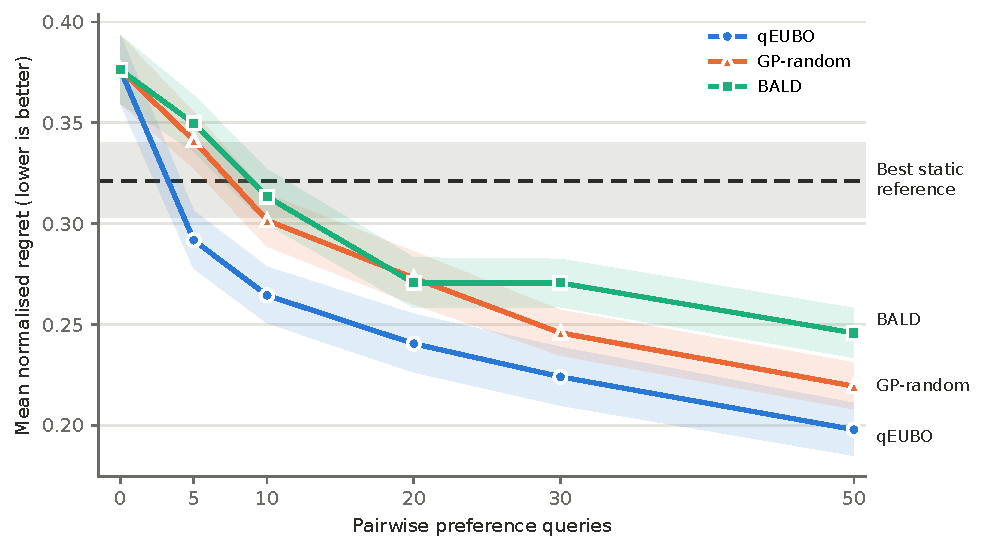
\includegraphics[width=0.92\linewidth]{fig2_learning_curves.pdf}
\caption{Mean normalised regret across the nine pre-specified cells as a function of pairwise preference budget, with 95\% listener-level bootstrap bands ($N=128$). The dashed line and grey band show the best static comparator (mean 0.3212). All learned policies share the same Laplace GP preference model.}
\label{fig:learning}
\end{figure}

Table~\ref{tab:curve} reports paired differences relative to the best static comparator. At $T=5$, the qEUBO interval already lies entirely below zero ($-0.0294$, 95\% CI $[-0.0470,-0.0123]$). The difference grows to $-0.1234$ at $T=50$.

\begin{table}[!htbp]
\centering
\caption{Paired listener-level differences in normalised regret relative to the best static comparator. Negative values favour the learned method.}
\label{tab:curve}
\begin{tabular}{rrrrrrr}
\toprule
 & \multicolumn{6}{c}{Query budget} \\
\cmidrule(lr){2-7}
Method & 0 & 5 & 10 & 20 & 30 & 50 \\
\midrule
qEUBO & +0.0551 & -0.0294 & -0.0568 & -0.0807 & -0.0972 & -0.1234 \\
BALD & +0.0551 & +0.0285 & -0.0079 & -0.0506 & -0.0506 & -0.0754 \\
GP-random & +0.0551 & +0.0201 & -0.0196 & -0.0482 & -0.0754 & -0.1018 \\
\bottomrule
\end{tabular}
\end{table}

\subsection{Acquisition efficiency}

The matched qEUBO-versus-GP-random comparison isolates active query selection from GP fitting. At five queries, qEUBO reduced regret by $0.0495$ relative to GP-random (95\% CI $[-0.0627,-0.0364]$). At ten queries, the difference was $-0.0371$ (95\% CI $[-0.0489,-0.0252]$). These two contrasts were pre-specified.

The exploratory extension to every budget (Table~\ref{tab:acq}) shows that the gap narrows but persists. It falls from about 0.05 at five queries to about 0.02 at 30 and 50 queries, where the interval still excludes zero. At $T=50$, mean regrets are 0.1978 for qEUBO and 0.2194 for GP-random. qEUBO also outperformed BALD at every budget. BALD's identical mean regret at $T=20$ and $T=30$ (0.2706) is coincidental: its recommendation changed between those budgets in 97.7\% of primary cells.

\begin{table}[!htbp]
\centering
\caption{Matched acquisition differences in normalised regret (listener-level 95\% bootstrap CIs; pre-specified families). Only qEUBO$-$GP-random at $T=5$ and $T=10$ was pre-specified; other entries are exploratory. The last row counts listeners for whom qEUBO had lower regret than GP-random.}
\label{tab:acq}
\resizebox{\linewidth}{!}{%
\begin{tabular}{@{}lccccc@{}}
\toprule
 & $T=5$ & $T=10$ & $T=20$ & $T=30$ & $T=50$ \\
\midrule
qEUBO$-$GP-random & $-0.049$ & $-0.037$ & $-0.033$ & $-0.022$ & $-0.022$ \\
 & $[-0.063,-0.036]$ & $[-0.049,-0.025]$ & $[-0.044,-0.021]$ & $[-0.034,-0.009]$ & $[-0.032,-0.011]$ \\
\addlinespace
qEUBO$-$BALD & $-0.058$ & $-0.049$ & $-0.030$ & $-0.047$ & $-0.048$ \\
 & $[-0.071,-0.045]$ & $[-0.062,-0.036]$ & $[-0.043,-0.017]$ & $[-0.059,-0.033]$ & $[-0.061,-0.035]$ \\
\addlinespace
\multicolumn{1}{@{}l}{qEUBO better than GP-random} & 93/128 & 90/128 & 90/128 & 79/128 & 89/128 \\
\bottomrule
\end{tabular}%
}
\end{table}

\subsection{Heterogeneity across contexts and preference families}

The primary $T=20$ effect varies by context (Fig.~\ref{fig:effects}, left). Noisy conversation shows a mean difference of $-0.1102$ (95\% CI $[-0.1331,-0.0873]$) and lecture $-0.1124$ (95\% CI $[-0.1415,-0.0835]$). Music is weaker at $-0.0197$, with a CI of $[-0.0443,+0.0047]$ that includes zero.

Effects also vary by preference family (Fig.~\ref{fig:effects}, right). Comfort shows the largest improvement, $-0.1848$ (95\% CI $[-0.2171,-0.1533]$). The balanced family improves by $-0.0458$ (95\% CI $[-0.0745,-0.0176]$). Intelligibility averaged across contexts is $-0.0117$ (CI $[-0.0420,+0.0189]$), giving no clear aggregate advantage at $T=20$.

\begin{figure}[!htbp]
\centering
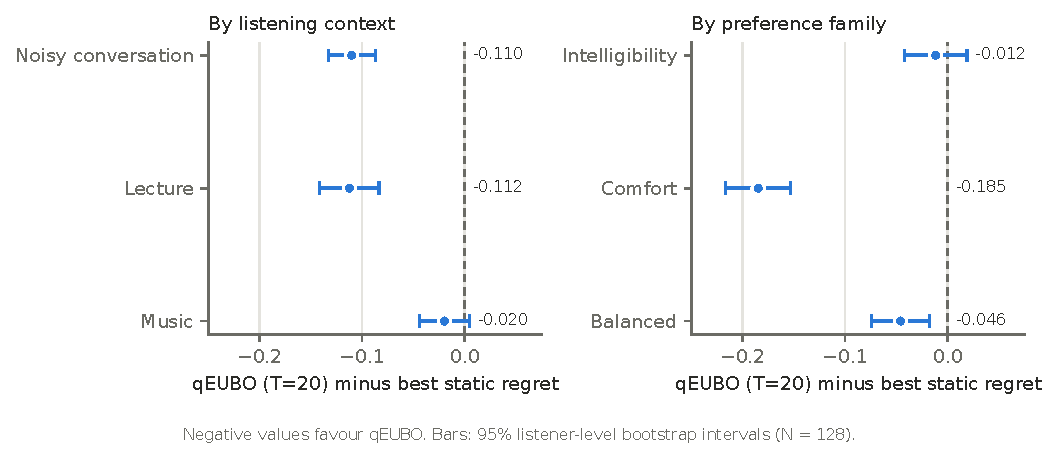
\includegraphics[width=\linewidth]{fig3_effects.pdf}
\caption{qEUBO ($T=20$) minus per-cell best static regret by listening context (left) and preference family (right). Error bars are 95\% listener-level bootstrap intervals. Negative values favour qEUBO.}
\label{fig:effects}
\end{figure}

\subsection{Context-by-family analysis}

Figure~\ref{fig:heatmap} and Table~\ref{tab:cells} show the interaction behind these aggregates. qEUBO improves all three preference families in noisy conversation and lecture. In music, comfort still improves strongly ($-0.1345$), balanced is essentially neutral ($+0.0001$), and intelligibility favours the static comparator ($+0.0754$, 95\% CI $[+0.0371,+0.1132]$). Section~\ref{sec:nrse} analyses this cell.

\begin{figure}[!htbp]
\centering
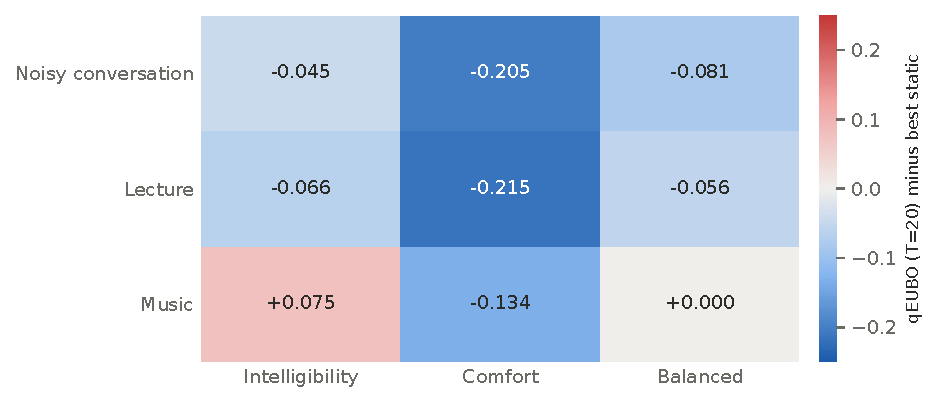
\includegraphics[width=0.84\linewidth]{fig4_context_family_heatmap.pdf}
\caption{Context-by-family mean paired difference for qEUBO at $T=20$ versus best static. Negative values (blue) favour qEUBO; positive values (red) favour static fitting.}
\label{fig:heatmap}
\end{figure}

\begin{table}[!htbp]
\centering
\caption{Context-by-family qEUBO $T=20$ differences versus best static.}
\label{tab:cells}
\begin{tabular}{llrr}
\toprule
Context & Family & Mean difference & 95\% CI \\
\midrule
Noisy conversation & Intelligibility & -0.0448 & $[-0.0833,-0.0063]$ \\
Noisy conversation & Comfort & -0.2046 & $[-0.2386,-0.1706]$ \\
Noisy conversation & Balanced & -0.0811 & $[-0.1166,-0.0461]$ \\
Lecture & Intelligibility & -0.0656 & $[-0.1051,-0.0260]$ \\
Lecture & Comfort & -0.2152 & $[-0.2607,-0.1709]$ \\
Lecture & Balanced & -0.0564 & $[-0.0963,-0.0164]$ \\
Music & Intelligibility & +0.0754 & $[+0.0371,+0.1132]$ \\
Music & Comfort & -0.1345 & $[-0.1646,-0.1048]$ \\
Music & Balanced & +0.0001 & $[-0.0358,+0.0368]$ \\
\bottomrule
\end{tabular}
\end{table}

\subsection{Post-hoc noise-sensitive robustness family}

The noise-sensitive family was introduced after a development diagnostic and cannot support the primary claim. It is nevertheless informative as a harder robustness case. qEUBO remains worse than static at $T=5$ ($+0.0633$, 95\% CI $[+0.0339,+0.0922]$) and $T=10$ ($+0.0300$, CI $[+0.0000,+0.0590]$), is indistinguishable at $T=20$ and $T=30$, and becomes clearly better only at $T=50$ ($-0.0446$, CI $[-0.0738,-0.0158]$). This contrasts with the pre-specified population, where qEUBO is already superior by five queries.

\section{Post-hoc exploratory analyses}
\label{sec:exploratory}

After the frozen final analysis, exploratory analyses were run to probe the mechanisms behind the main results. New simulations used only development seed 424242; analyses of the final cohort re-read the released rows without running any new simulation. None of these analyses can alter the pre-specified estimand, and their intervals are descriptive. Scripts and outputs are released under \texttt{scripts/} and \texttt{publication/postfinal\_diagnostics/}.

\subsection{A simple interactive baseline}

A model-free coordinate-search baseline compares the current setting with a single-coordinate step, keeps the preferred setting, and halves the step after each sweep. On the 32-listener development sweep at 20 queries, its listener-mean regret difference relative to the static reference was $+0.0275$ (worse than static), and it beat static for 11/32 listeners. On the same listeners qEUBO was $-0.0566$ relative to static and beat static for 21/32. Interaction alone therefore does not reproduce the gain of the GP-based active policy at this budget.

\subsection{Query geometry}

A query endpoint was labelled ``near boundary'' when $\max_j |z_j|\geq0.9$. Across 32 development listeners, nine primary cells and the first 30 queries, 87.6\% of BALD endpoints were near the boundary, compared with 22.9\% for qEUBO. The information-gain objective thus spends many comparisons on extreme settings. This is consistent with BALD's weaker performance throughout Table~\ref{tab:acq}, although the diagnostic does not establish causality.

\subsection{Why music--intelligibility favours static fitting}
\label{sec:nrse}

Three observations, combining the released final rows with a development-seed diagnostic (32 listeners, intelligibility family, $T=20$; Table~\ref{tab:nrse}), account for the music--intelligibility result.

First, the corner optimum is built into the oracle. In music, noise reduction and speech enhancement offer no benefit and carry a doubled artefact cost (Section~\ref{sec:oracle}), so the optimum has both switched off ($z_4=z_5=-1$); every final music--intelligibility optimum lies at that corner.

Second, the learner hardly moves these two controls in any context. In the final cohort, the mean $z_4$ of qEUBO's $T=20$ recommendations lies between $-0.21$ and $+0.09$ in every primary cell, whereas the optimum sits near $z_4=-1.00$ in all music cells and near $+0.69$ in noisy-conversation--intelligibility. Only 3.9\% of music--intelligibility recommendations reach the enhancement-off corner at $T=20$ (1.6\% at $T=50$). The development diagnostic shows why. The hidden utility carried by $z_4$ and $z_5$---the loss from resetting them to their prescription values at the optimum---has a median of only 0.10, 0.18 and 0.46 choice-noise standard deviations in lecture, music and noisy conversation, respectively. A few dozen noisy comparisons cannot resolve differences that small. Removing response noise lowered qEUBO regret in every intelligibility cell, not only in music, so noise is a general limit rather than a music-specific cause. Adding the exact enhancement-off corner to every candidate pool changed no recommendation (32 of 32 listeners), and setting the prior coefficient $\gamma$ to zero increased music--intelligibility regret from 0.294 to 0.382.

Third, one static comparator---the linear setting---sits exactly at the music corner. It is the better static choice in 71\% of final music--intelligibility cells, against 47\% of all primary cells. The music--intelligibility deficit therefore reflects an unusually strong static reference in a cell whose optimum lies along low-stake controls, rather than a music-specific failure of the learner.

\begin{table}[!htbp]
\centering
\caption{Development-seed diagnostic of the noise-reduction/speech-enhancement controls (32 listeners, intelligibility family, qEUBO at $T=20$). Stake: median loss of hidden utility when $z_4,z_5$ are reset to 0 at the optimum, in units of the listener's choice-noise standard deviation. Regrets are means; $z_4$ columns give the mean recommended and optimal noise-reduction coordinate.}
\label{tab:nrse}
\small
\begin{tabular}{@{}lcccccc@{}}
\toprule
 & & \multicolumn{3}{c}{Mean regret} & \multicolumn{2}{c}{Mean $z_4$} \\
\cmidrule(lr){3-5}\cmidrule(l){6-7}
Context & Stake & Static & qEUBO & Noise-free & Rec. & Opt. \\
\midrule
Noisy conversation & 0.46 & 0.379 & 0.347 & 0.082 & $+0.06$ & $+0.53$ \\
Lecture & 0.10 & 0.329 & 0.249 & 0.042 & $-0.17$ & $-0.19$ \\
Music & 0.18 & 0.256 & 0.294 & 0.069 & $-0.05$ & $-1.00$ \\
\bottomrule
\end{tabular}
\end{table}

\subsection{Robustness to oracle and observation assumptions}
\label{sec:robust}

A development-only sweep re-ran qEUBO and GP-random at $T=20$ under perturbed oracle and observation assumptions for 32 listeners, with both policies sharing each listener's seeds (Table~\ref{tab:robust}). Under the frozen assumptions, qEUBO improved on the static reference by $-0.056$ (95\% CI $-0.120$ to $-0.001$; 19 of 32 listeners), in the same direction as the final-cohort estimate, and on GP-random by $-0.017$ ($-0.040$ to $+0.006$).

The advantage over static fitting persisted, and grew, when the listener-specific ideal-gain offsets were doubled ($-0.113$) or the ideal-gain term was removed altogether ($-0.181$). It remained negative under doubled audiogram-measurement error ($-0.070$), where six of 32 draws had no feasible low-gain anchor; these were recorded as infeasible rather than repaired by relaxing constraints. Doubling choice noise and lapse rates reversed the picture. qEUBO minus static became $+0.039$ ($-0.016$ to $+0.088$), with only 9 of 32 listeners better than static, a within-listener shift of $+0.095$ ($+0.071$ to $+0.121$) from the base scenario. Under the same high-noise condition qEUBO also lost its edge over GP-random ($+0.014$, $-0.014$ to $+0.043$). The qualitative conclusions therefore do not hinge on the ideal-gain construction, but they do depend on how reliably the simulated listener answers.

\begin{table}[!htbp]
\centering
\caption{Development-only robustness sweep (seed 424242; qEUBO and GP-random at $T=20$; listener-level 95\% bootstrap CIs). $n$: listeners with a feasible low-gain anchor. Negative differences favour qEUBO.}
\label{tab:robust}
\resizebox{\linewidth}{!}{%
\begin{tabular}{@{}lcccc cc@{}}
\toprule
Scenario & $n$ & \multicolumn{2}{c}{qEUBO $-$ static} & & \multicolumn{2}{c}{qEUBO $-$ GP-random} \\
\cmidrule(lr){3-4}\cmidrule(l){6-7}
 & & Mean [95\% CI] & Better & & Mean [95\% CI] & Better \\
\midrule
Base (frozen assumptions) & 32 & $-0.056$ $[-0.120, -0.001]$ & 19/32 & & $-0.017$ $[-0.040, +0.006]$ & 23/32 \\
Ideal-gain offsets doubled & 32 & $-0.113$ $[-0.172, -0.055]$ & 23/32 & & $-0.026$ $[-0.053, +0.001]$ & 20/32 \\
Audiogram error doubled ($\sigma_a=10$ dB) & 26 & $-0.070$ $[-0.148, -0.005]$ & 16/26 & & $-0.025$ $[-0.059, +0.008]$ & 15/26 \\
Ideal-gain term removed & 32 & $-0.181$ $[-0.244, -0.126]$ & 29/32 & & $-0.053$ $[-0.079, -0.027]$ & 25/32 \\
Choice noise and lapses doubled & 32 & $+0.039$ $[-0.016, +0.088]$ & 9/32 & & $+0.014$ $[-0.014, +0.043]$ & 15/32 \\
\bottomrule
\end{tabular}%
}
\end{table}

\section{Discussion}
\label{sec:discussion}

\subsection{Main finding: decision-theoretic feedback selection improves low-budget closed-loop control}

The principal result is not simply that a GP can learn a simulated listener preference. Prior hearing-aid work already demonstrates that pairwise comparisons and Bayesian models can support personalisation \cite{birlutiu2010,nielsen2015,vyas2022,ni2024}. The stronger result is that, under matched modelling conditions, \emph{which comparisons are requested} materially changes the recommendation quality at small budgets.

At five queries, qEUBO is already better than the strengthened static reference, while BALD and GP-random remain worse than static on average. qEUBO also beats GP-random directly by about 0.05 normalised-regret units. As the budget grows the gap narrows but does not close: random exploration progressively supplies the GP with useful coverage, while qEUBO places early queries where they most improve the terminal recommendation and retains a smaller advantage throughout. BALD, which targets information about the whole preference function, spends much of its budget near the boundary of the latent space (Section~\ref{sec:exploratory}) and trails both alternatives at most budgets.

This distinction matters for closed-loop biomedical and assistive systems. A perceptual comparison is a feedback measurement, but it is not free: it consumes attention, can induce fatigue and may become less reliable with repeated exposure. The practical control objective is therefore a useful device recommendation after a small number of measurements rather than asymptotic recovery of the entire preference function. qEUBO is aligned with that objective because it chooses feedback specifically for its expected value to the terminal recommendation.

\subsection{Strength of the static comparator}

The primary analysis takes the per-cell minimum across three recorded static rows, but only two distinct primary utility behaviours are represented. The default and slow rows have identical utility because compression speed is absent from the three pre-specified primary families. The linear row is more than a compression-only alternative: it also switches noise reduction and speech enhancement off. The static reference should therefore be understood as the better of two distinct synthetic static behaviours, not as three independent prescriptions.

This reference is still stronger than the default half-gain setting alone, because each cell may retrospectively choose between the default behaviour and the linear, enhancement-off behaviour. It is the better choice in 47\% of primary cells and in 71\% of music--intelligibility cells.

\subsection{Why comfort is easier to improve than intelligibility}

The large comfort effect and smaller intelligibility effect are plausible given the problem construction and the application domain. A prescription rule is designed to supply audibility and speech-oriented gain from audiometric information, so there may be less room for preference optimisation when the hidden objective is dominated by an intelligibility-like term.

Comfort is more idiosyncratic. Listener-specific upper limits, preferred gain offsets and processing penalties create heterogeneous optima that cannot be recovered from the audiogram alone, so pairwise preference learning has more to add. This pattern is consistent with self-fitting studies showing that user-selected settings often remain near prescription-derived solutions while exhibiting systematic individual deviations \cite{dreschler2008,sabin2020}.

\subsection{Contexts and low-stake controls}

Noisy conversation and lecture show robust qEUBO gains, whereas music is weak overall because of the music--intelligibility cell. The analysis in Section~\ref{sec:nrse} suggests a more general lesson than a music-specific failure. Controls whose effect on utility is small relative to response noise---here noise reduction and speech enhancement---are barely moved by a few dozen noisy comparisons in any context. When a static comparator happens to sit at the optimum of such a control, as the linear setting does in music, the learner cannot catch up within the budget. Future systems could address this with automatic relevance determination kernels, context-conditioned or multi-task models \cite{birlutiu2010}, or queries that vary one low-stake control at a time.

\subsection{Response reliability}

The robustness sweep (Section~\ref{sec:robust}) shows that the advantage over static fitting depends on how reliable the simulated preferences are. Static fitting does not use responses, so noisier responses can only hurt the learner. With doubled choice noise and lapse rates, the best static setting was no longer outperformed at 20 queries, and qEUBO no longer outperformed random pair selection. This is consistent with evidence that listeners' preferences for gain adjustments depend on how much speech they hear before judging \cite{whitmer2022}. Response reliability should therefore be measured, and ideally modelled, in any human study.

\subsection{Relation to recent hearing-aid ML}

Nielsen et al. \cite{nielsen2015} already demonstrated GP active learning from pairwise perceptual comparisons in hearing-aid parameter adjustment, and Korzepa et al. \cite{korzepa2020} developed a simulation environment for contextual hearing-aid personalisation. Reinforcement-learning approaches have personalised compression from user feedback \cite{alamdari2020,akbarzadeh2022}. Vyas et al. \cite{vyas2022} demonstrated efficient pairwise identification over a discrete preset set, and Ni et al. \cite{ni2024} improved training efficiency through multi-band Bayesian learning with a small clinical validation.

AudioTwin differs mainly in its closed-loop systems emphasis. It treats audiometric measurements as the conditioning biomedical input, behavioural pairwise choices as the feedback signal, and multidimensional DSP settings as the controlled device variables. The final evaluation is a controlled acquisition-policy comparison with a frozen protocol, explicit feasibility projection and an oracle-strengthened static baseline. This design asks whether a feedback-selection policy improves the quality of assistive-device recommendations under limited interaction budgets without treating simulated utility as clinical evidence.

\subsection{Feasibility constraints and the rejected listener}

One simulated listener in the final draw admitted no feasible low-gain anchor under the frozen constraints. Rather than weakening constraints after observing the failure, the task was recorded as infeasible and replaced using a deterministic rule defined before performance analysis. An algorithm should be allowed to fail closed when the assumed feasible domain is empty. In a real hearing-care workflow, the corresponding response would not be automatic relaxation of model limits but fallback to a verified configuration, additional measurement or professional review. These constraints are computational guardrails and should not be equated with regulatory or clinical safety guarantees.

\subsection{Protocol discipline as part of applied ML evaluation}

Applied optimisation studies are vulnerable to researcher degrees of freedom. Candidate spaces, baselines, oracle definitions, budgets and random seeds can all be changed after preliminary results are seen. Such adaptation may be necessary during development, but it weakens confirmatory interpretation if the same outcomes are repeatedly reused.

AudioTwin records development/final separation in its protocol history. A reserved final seed was not used during method development, and the primary endpoint, sample size and bootstrap procedure were specified before final outcomes were inspected. A compression artefact discovered during development was not inserted into the three pre-specified utility families but isolated in a post-hoc robustness family. The original development branch and annotated tags are public, although they remain repository provenance rather than an externally registered protocol. These choices do not eliminate all design bias---the simulator itself was developed by the author---but they reduce direct tuning to the reported final random draw.

\section{Limitations}
\label{sec:limitations}

\subsection{Simulation is not clinical validation}

The most important limitation is that all 128 final listeners are simulated. The oracle contains plausible ingredients---audibility, comfort, ideal-gain deviation, compression preference and response noise---but it is not a human participant. Lower oracle regret demonstrates successful optimisation of the specified benchmark, not improved hearing outcomes. Because recent hearing-aid personalisation studies include real participant data \cite{vyas2022,akbarzadeh2022,ni2024}, AudioTwin should therefore be viewed as a methodological closed-loop simulation and reproducibility study that motivates, rather than replaces, a human-listener trial with measured acoustic outputs and clinically relevant outcomes.

\subsection{The oracle and learner share structural assumptions}

Although the oracle is not exposed to the learner, both are smooth functions over the same latent DSP space, and the oracle's hidden ideal gain is derived from the same half-gain prescription used by the learner, plus random listener-specific offsets. These shared assumptions favour smooth preference learning and limit external validity. Real preferences may include discontinuities, hysteresis, context drift, adaptation and non-stationary judgement noise. The development-only robustness checks in Section~\ref{sec:robust} probe some of these assumptions but cannot replace a differently constructed oracle or human data.

\subsection{Sensitivity to response noise}

When simulated choice noise and lapse rates were doubled, the advantage over static fitting reversed and the advantage over random pair selection disappeared. The size of any benefit in practice will therefore depend on how consistently real listeners can judge the presented pairs.

\subsection{Approximate optimum and normalised regret}

The oracle optimum is computed numerically by random-plus-evolutionary search specified in the frozen experiment, so regret is measured relative to an approximate feasible optimum. This is suitable for comparing methods under the same benchmark but introduces numerical approximation error into the absolute regret scale.

\subsection{Known rather than learned constraints}

AudioTwin projects candidates against known model constraints. It does not infer safety from observations and therefore does not solve the full safe-BO problem addressed by methods such as SafeOpt \cite{sui2015}. Applications with uncertain constraints would require a probabilistic constraint model and a different safety analysis.

\subsection{Limited signal-processing and context model}

The six-dimensional latent space omits many commercial hearing-aid features, including binaural coordination, adaptive directionality, feedback cancellation, source separation and modern neural speech enhancement. The three final contexts cover only a small subset of real environments. The reported effects should not be extrapolated to a complete hearing-aid signal chain.

\subsection{No computational-time or human-fatigue outcome}

The study counts preference comparisons but does not model response time, fatigue or cognitive burden. Pairwise queries with similar candidates may be information-rich yet perceptually difficult. Human studies should jointly optimise statistical efficiency and usability.

\section{Future work}
\label{sec:future}

The highest-priority next step is a prospective listening study in which the optimisation loop controls an implemented hearing-aid signal-processing chain and each candidate setting is evaluated using reproducible acoustic stimuli. A suitable initial design would compare a verified prescription, conventional fine-tuning and AudioTwin-qEUBO within participants. Outcomes should include preference, speech recognition in noise, comfort, listening effort, test--retest stability and the number of comparisons required to reach a stable setting. Stimulus duration should be chosen with reference to evidence that preference reliability depends on the amount of speech presented \cite{whitmer2022}.

A second direction is hierarchical preference learning. Preference structure can be shared across listeners \cite{birlutiu2010}; a population prior could reduce cold-start queries while retaining individual adaptation.

A third direction concerns low-stake controls and context transfer. Automatic relevance determination, multi-task kernels that share strength between speech contexts while letting music keep a distinct latent function, and noise-aware acquisition are all directly testable against the music--intelligibility and response-noise results reported here.

Finally, learned constraints and modern neural audio processing could be integrated. The optimisation layer could tune parameters of speech-enhancement or source-separation systems, while a probabilistic safety and quality model excludes settings with unacceptable distortion.

\section{Conclusion}
\label{sec:conclusion}

AudioTwin treats hearing-aid fine-tuning as a constrained engineering optimisation problem that combines audiogram information with a small number of listener preference choices. In the frozen evaluation of 128 simulated listeners, qEUBO reduced mean normalised regret from 0.3212 for the best static comparator to 0.2405 after 20 pairwise choices, a 25.1\% reduction. The method improved on the static reference for 94 of 128 simulated listeners.

The matched random comparison shows why the query-selection policy matters. Using the same GP preference model, targeted qEUBO comparisons produced better recommendations than random comparisons at the pre-specified five- and ten-query budgets. This means the improvement was not caused only by fitting a preference model; it also depended on asking more useful questions.

For real-world hearing technology, the potential benefit is a fitting process that learns personal preference with fewer unnecessary adjustments. Such a system could support clinicians by narrowing the search for a preferred setting, and it could provide a basis for guided self-fitting where appropriate. It may also help a device adapt settings to different listening contexts instead of relying on one fixed configuration. These benefits remain prospective. The current study is simulation-based, the constraints are model-based engineering guardrails rather than certified safety limits, and human-listener studies with measured acoustic outputs are required before clinical benefit can be claimed.

\section*{CRediT authorship contribution statement}
Anonymous Author: Conceptualisation, Methodology, Software, Validation, Formal analysis, Investigation, Data curation, Visualisation, Writing -- original draft, Writing -- review \& editing, Project administration.

\section*{Funding}
This research did not receive any specific grant from funding agencies in the public, commercial, or not-for-profit sectors.

\section*{Declaration of competing interest}
The author declares no known competing financial interests or personal relationships that could have appeared to influence the work reported in this paper.

\section*{Ethics statement}
The reported evaluation is a computational simulation and did not recruit human participants or use identifiable participant data. Human-participant ethics approval was therefore not required for the experiments reported here. Any prospective human-listener validation will require appropriate institutional ethics review and informed consent.

\section*{Data and code availability}
The AudioTwin source code, released final dataset, analysis scripts, protocol records and LaTeX manuscript sources are provided through an anonymised supplementary repository for peer review under the MIT License; the Results in Engineering submission snapshot corresponds to tag \path{manuscript-rineng-v1.1}. The file \path{publication/data/final_v1.parquet} contains all 32,256 final analysis rows. \path{scripts/analyze_final.py} recomputes the primary and pre-specified secondary results from it, \path{scripts/make_publication_summaries.py} regenerates the context/family summaries and figure inputs, and \path{scripts/analyze_exploratory_final.py} produces the exploratory final-cohort analyses. Development-seed diagnostic scripts and outputs are in \path{scripts/} and \path{publication/postfinal_diagnostics/}. Exact package versions from the final-run environment are pinned in \path{requirements-final.txt}. The curated \path{main} history is post-experiment; the original development lineage and annotated protocol tags are published on the \path{protocol-history} branch and documented in \path{PROTOCOL_PROVENANCE.md}.

\section*{Declaration of generative AI and AI-assisted technologies in the manuscript preparation process}
During the preparation of this work, the author used ChatGPT (OpenAI) solely to improve
the grammar, language, clarity and readability of the manuscript. The tool was not used for
research design, data generation, simulation, implementation, data analysis, interpretation of
results, or formulation of scientific conclusions. After using this tool, the author reviewed and
edited the content as needed and takes full responsibility for the content of the publication.


\section*{Acknowledgements}
The author acknowledges the computational resources and institutional research support used for the final simulation experiments. Identifying institutional details have been withheld for anonymous peer review.

\appendix

\section{Oracle equations}
\label{app:oracle}

DSP settings are computed from the estimated audiogram $\hat a_l$, whereas thresholds, comfort limits and the ideal gain use the listener's true audiogram. For DSP band $k$, let $L_k$ be the long-term speech level in the context, $g_k$ and $CR_k$ the gain and compression ratio, $T_k$ the true threshold in dB SPL, $U_k$ the upper comfort limit and $I_k$ a band-importance weight ($\sum_k I_k=1$). The compressed speech output is
\begin{equation}
 O_k=\min\!\big(L_k+g_k-(1-1/CR_k)\max(L_k-45,0),\ 105\big)\ \text{dB SPL}.
\end{equation}
With noise-reduction and speech-enhancement strengths $\mathrm{NR}=(z_4+1)/2$ and $\mathrm{SE}=(z_5+1)/2$ and context benefits $B_{\mathrm{NR}}$, $B_{\mathrm{SE}}$ (3/4~dB in noisy conversation, 2/3~dB in lecture, 0 in music), the output SNR is $\mathrm{SNR}_{\mathrm{out}}=\mathrm{SNR}+B_{\mathrm{NR}}\mathrm{NR}+B_{\mathrm{SE}}\mathrm{SE}$. The four components are
\begin{align}
 A &= \textstyle\sum_k I_k\,\mathrm{clip}\!\left(\frac{\min(\mathrm{SNR}_{\mathrm{out}},\,O_k+12-T_k)+15}{30},0,1\right),\\
 c &= \tfrac{1}{K}\textstyle\sum_k \big(2d_k^2\,[d_k>0]+d_k^2\,[d_k\le0]\big)\nonumber\\
   &\quad+\tfrac{1}{K}\textstyle\sum_k \big(\max(O_k+12-U_k,0)/5\big)^2,\qquad d_k=\big(O_k-\tfrac{T_k+U_k}{2}\big)/10,\\
 D &= \tfrac{1}{K}\textstyle\sum_k\big((g_k-g^{ideal}_{l,k})/10\big)^2,\\
 Q &= w_{\mathrm{art}}\big(0.5\,\mathrm{NR}^2+0.7\,\mathrm{SE}^2\big)+\big(\log_2\overline{CR}-\rho_l\big)^2,
\end{align}
with $K=10$ bands, $\overline{CR}$ the mean compression ratio, $\rho_l\sim U(0,1)$ the listener's preferred $\log_2$ compression ratio, and $w_{\mathrm{art}}=1$ in speech contexts and 2 in music. Then $P_C=\mathrm{pen}(c)$, $P_D=\mathrm{pen}(D)$ and $P_Q=\mathrm{pen}(Q)$ with $\mathrm{pen}(x)=1-e^{-x}$. Family weights $(w_A,w_C,w_D,w_Q)$ are drawn per listener from Dirichlet distributions with concentrations $(6,1,1,1)$ for intelligibility, $(1,5,2,1)$ for comfort and $(3,3,2,2)$ for balanced. The post-hoc noise-sensitive family uses $(4,2,1,3)$ and adds $3.0\,n\,(\log_2\overline{CR})^2+1.5\,n\,s\,(\log_2\overline{CR})^2$ to $Q$, where $n=\mathrm{clip}((15-\mathrm{SNR})/15,0,1)$ and $s$ is 1 at the fast and 0 at the slow attack time on a logarithmic scale. Because $B_{\mathrm{NR}}=B_{\mathrm{SE}}=0$ and $w_{\mathrm{art}}=2$ in music, the music optimum has $\mathrm{NR}=\mathrm{SE}=0$.

\bibliographystyle{elsarticle-num}
\bibliography{references}

\end{document}
